\documentclass[article,fleqn,12pt]{article}

\usepackage{amsmath, amssymb, amsfonts}
\usepackage{tikz, pgfplots}
\usepackage{enumitem}

\usepackage{scalerel,stackengine}
\newcommand\equalhat{\mathrel{\stackon[1.5pt]{=}{\stretchto{%
\scalerel*[\widthof{=}]{\wedge}{\rule{1ex}{3ex}}}{0.5ex}}}}

\pgfplotsset{compat=1.18}
\usepgfplotslibrary{colorbrewer}

\DeclareMathOperator{\sign}{sign}

\begin{document}

\subsection{Preliminaries}
\bgroup
\renewcommand{\arraystretch}{1.5}
\begin{tabular}{l p{8cm}}
\(w, h \in \left[\!\left[1,50\right]\!\right]\) & width and height of the map, respectively. \\
\(T := \left[\!\left[0,w-1\right]\!\right] \times \left[\!\left[0,h-1\right]\!\right]\) & set of all tiles. \\
\(P \in \bigcup^7_{i=1}\left[\!\left[0,i\right]\!\right]\) & set of all players. \\
\(L := P \,\cup\, \left\{\,\text{H},\,\text{B},\,\text{C},\,\text{I},\,\text{X}\,\right\}\) & set of all tile types. \\
\(\ell : L \to 2^T\) & map of each tile type to a set of tiles, where \(\forall l_1, l_2 \in L,\,l_1 \neq l_2: \ell(l_1)\,\cap\,\ell(l_2) = \emptyset\) \\
\(i_{\text{o}}: P \to \left[\!\left[0,255\right]\!\right]\) & map of each player to a number of override stones. \\
\(i_{\text{b}}: P \to \left[\!\left[0,255\right]\!\right]\) & map of each player to a number of bombs.
\end{tabular}
\egroup

\vspace{15px}

\subsection{Approximating the remaining move count}
The temporal aspect of a board's configuration is relevant for the appropriate evaluation of a player's position. More precisely, the amount of remaining moves must influence heuristic evaluation. We define a move identification value (\textbf{move no.}) as the ordinal position of a configuration within the overall sequence of game states. For the proper estimation of the remaining move count, provided an arbitrary (but valid) game state, the following upper bound is proposed: 
\begin{align*}
& m_{\text{upper}} := \underbrace{wh - \left|\ell(\text{H})\right|}_{\text{unoccupied tiles}} + \left|\ell(\text{B})\right| + \sum_{p \in P} i_{o}(p) + i_{b}(p) - \left|\ell(p)\right|.
\end{align*} \\[-1em]

To evaluate the reliabilty of this upper bound, we conducted the following experiment for a multitude of maps: At each turn of player \(p\), we output the computed upper bound for the remaining move count. The recorded predictions are compared to the actual remaining move count post-game. While on the majority of tested maps the upper bound corresponded to the remaining move count precisely, the gap between the two values showed a minor margin of error during early phases on some game instances. The following plot displays these outliers and the slight inaccuracies:
\pagebreak

\begin{figure}
\centering
\begin{tikzpicture}[scale=0.8]
  \begin{axis}[
		/pgf/number format/.cd,
			1000 sep={},
		xlabel={Move no.},
ylabel={Accuracy (\(100\% - \frac{m_{\text{upper}} - \left(\text{total move count} - \textbf{move no.}\right)}{m_{\text{upper}}}\))},
		ylabel style={rotate=-90, anchor=south west, yshift=95},
		yticklabel={\pgfmathparse{\tick*100}\pgfmathprintnumber{\pgfmathresult}\%},
		xmin=1,
		xmax=400,
		grid=both,
		width=12cm,
		height=8cm,
		legend style={at={(0.98,0.02)},anchor=south east}
	]
		\addplot[blue, thick] table [x=entry, y=accuracy, smooth, col sep=space] {data/move_approximation/2025_g1_1_twoplayer.txt};
		\addlegendentry{2025\_g1\_1\_twoplayer}
		\addplot[red, thick] table [x=entry, y=accuracy, smooth, col sep=space] {data/move_approximation/25_25_2_25_rnd_1.txt};
		\addlegendentry{25\_25\_2\_25\_rnd\_1}
  \end{axis}
\end{tikzpicture}
\caption{Accuracy of \(m_{\text{upper}}\)}
\label{fig:m_upper_accuracy}
\end{figure}
As the sparsity of possible legal moves increases, we except the accuracy to increase, which is indeed the case \ref{fig:m_upper_accuracy}. It is speculated that the early inaccuracies stem from override moves, however, we do not indent to further investigate this.

\vspace{15px}

\subsection{Stone-Counting Heuristic}
\subsubsection{Formula requirements}
Let \(p \in P\) be a fixed but arbitrary player whose position we want to evaluate based on stone count. The following heuristic is derived from the win condition of \textit{Reversi plus X}, which states that the player with the majority of stones on the board in the terminal state wins. The terminal state is defined as a bomb phase configuration, in which every player has no legal moves. \\\\
\underline{\textbf{Codomain:}} Let \(\left[\text{MIN},\,\text{MAX}\right] \subsetneq \mathbb{R}\) define the value space of our evaluation formula, where \(\text{MIN} \neq -\infty,\,\text{MAX} \neq \infty,\,\text{MIN} < \text{MAX}\). \\\\
\underline{\textbf{Domain:}} The \textbf{move no.}, \(\left|\ell(p)\right|\), and \(\max\left\{\ \left|\ell(o)\right|\ |\ o \in P \setminus p\ \right\} =: \left|\ell(o_1)\right|\) are input values for the evaluation function. Let S := \(\bigcup_{p\in P}\ell(p)\) denote the set of all player stones which are on the board. Then the function domain is defined as
\begin{align*} 
D := \underbrace{\left[\!\left[1, m_{\text{upper}}\right]\!\right]}_{\substack{\textbf{move no.}\\\text{value space}}} \times \underbrace{\left\{\, \left(p_1, p_2\right) \in \mathbb{N}_0^{2}\ |\ p_1 + p_2 \leq \left|S\right|\, \right\}}_{\left(\left|\ell(p)\right|,\,\left|\ell(o_1)\right|\right) \text{ value space}}.
\end{align*} \\
\underline{\textbf{Criteria:}}
\begin{enumerate}[label=(\roman*)]
\item Stone count distance is less significant during early game states, while evaluations must converge to appropriate extrema as the game progresses. 
\item A tie between stone counts of \(p\) and \(o_1\) must be attributed \(\frac{MAX + MIN}{2}\).
\item Independent of \textbf{move no.}, configurations where \(\ell(p) = \emptyset\) must be evaluated with MIN, and conversely, configurations where \(\ell(o_1) = \emptyset\) must always be attributed MAX. 
\end{enumerate}

\subsubsection{Formula construction}
In the following, we fix MAX to \(1\) and MIN to \(-\text{MAX}\). For criteria (i) and (ii), we define an interpolation \(f: D \to \left[-\text{MAX},\text{MAX}\right]\) as
\begin{align*}
f(t, p_1, p_2) := tm_{\text{upper}}^{-1}\sign(p_1 - p_2) + \left(1 - tm_{\text{upper}}^{-1}\right)\left(p_1 - p_2\right)\left|S\right|^{-1}.
\end{align*} \\
Condition (i) is met with \(\forall t: p_1 = p_2 \Rightarrow f(t, p_1, p_2) = \frac{MAX - MAX}{2} = 0\). As \(t\) approaches \(m_{\text{upper}}\) (corresponding to the game nearing the approximated terminal state), the left hand addend approaches -MAX or MAX, respectively, while the right hand addend approaches zero. Otherwise, the evaluation is based on the normalized stone count difference (ii). 

To emphasize urgency in early game scenarios, where stone counts are near zero, we define a scaling term \(h: \left\{\, \left(p_1, p_2\right) \in \mathbb{N}_0^{2}\ |\ p_1 + p_2 \leq \left|S\right|\, \right\} \to \left[-\text{MAX},\text{MAX}\right]\), where
\begin{align*}
h(p_1, p_2) := \left|p_1 - p_2\right|\left|S\right|^{-1}\left(1 + \min\left\{ p_1, p_2 \right\}\right)^{-1}.
\end{align*} \\
We then construct the function \(\mathfrak{A}: D \to \left[-\text{MAX},\text{MAX}\right]\), with 
\begin{align*}
\mathfrak{A}(t, p_1, p_2) := \begin{cases}
\quad -\text{MAX},& p_1 = 0 \lor p_2 = \left|S\right| \\
\quad \text{MAX},& p_2 = 0 \lor p_1 = \left|S\right| \\
\quad h(p_1, p_2)\sign(p_1 - p_2) & \text{otherwise} \\[-0.2em]
+ \, (1 - h(p_1, p_2))f(t, p_1, p_2),&
\end{cases}
\end{align*}
This function fulfills all criteria for our evaluation formula (i - iii).

\subsubsection{Graphing}
Given the classical reversi map...

\begin{center}
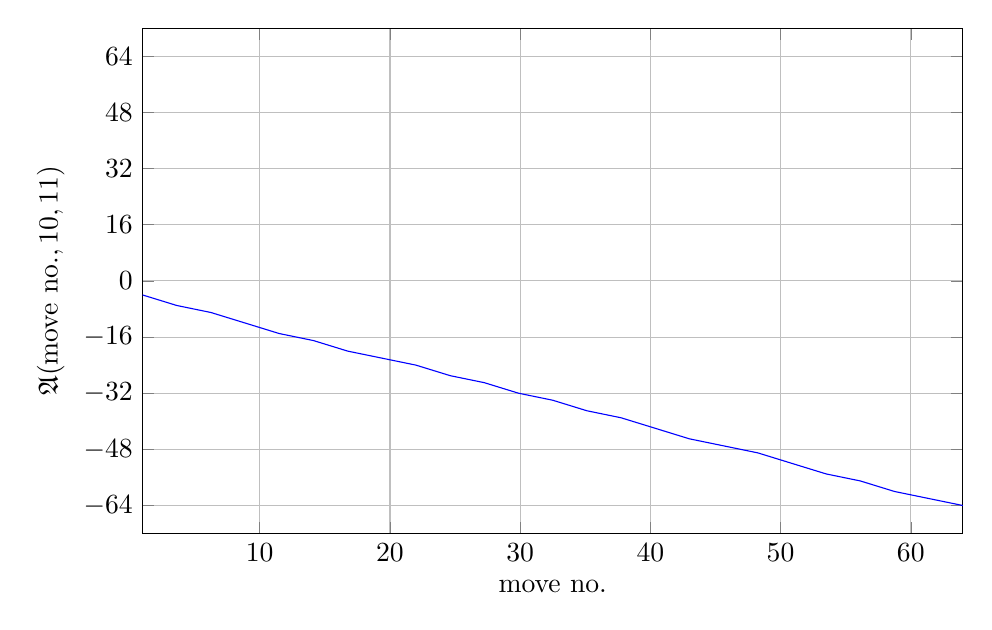
\begin{tikzpicture}
	\pgfmathsetmacro{\upper}{64}
	\pgfmathsetmacro{\p}{10}
	\pgfmathsetmacro{\o}{11}
	\pgfmathsetmacro{\k}{1}
	\pgfmathsetmacro{\MAX}{64}
	\pgfmathsetmacro{\h}{floor((\MAX * abs(\p - \o)) / ((\p + \o) * (1 + min(\p, \o))))}

  \begin{axis}[
		colormap/PuBu,
		/pgf/number format/.cd,
			1000 sep={},
		xlabel={move no.},
		ylabel={\(\mathfrak{A}(\text{move no.}, \p, \o)\)},
		xmin=1,
		xmax=\upper,
		ymin={\MAX * (-1.125)},
		ymax={\MAX * 1.125},
		ytick={-64, -48, -32, -16, 0, 16, 32, 48, 64},
		grid=both,
		width=12cm,
		height=8cm,
	]
		\addplot [blue, domain=1:\upper] {
		floor(\h * sign(\p - \o) + ((\MAX - \h) * ((((1 - (x / \upper)) * (\p - \o)) / (\p + \o)) + ((x * sign(\p - \o)) / \upper))))
  };
  \end{axis}
\end{tikzpicture}

\end{center}

\end{document}

